\begin{surferPage}[Quintic (15 Cusps)]{A Quintic with 15 Cusps}
  This surface of degree $5$ (quintic) has $15$ singularities of type $A_2$
    (called cusps); this quintic and a series of related surfaces was given in
    an article from 2005 by Oliver Labs.
    Five of the cusps differ in appearance from the other ten.
    Indeed, the five are $A_2^{++}$ singularities, the other $A_2^{+-}$ (see
    the gallery on simple singularities for more info):

     \vspace*{-0.3em}
    \begin{center}
      \begin{tabular}{c@{\qquad}c}
        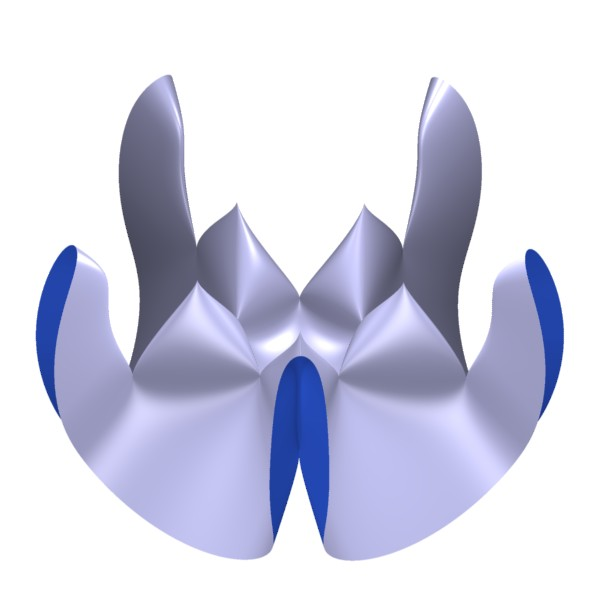
\includegraphics[height=1.2cm]{./../../common/images/dessins_quint_15a2}
        &
        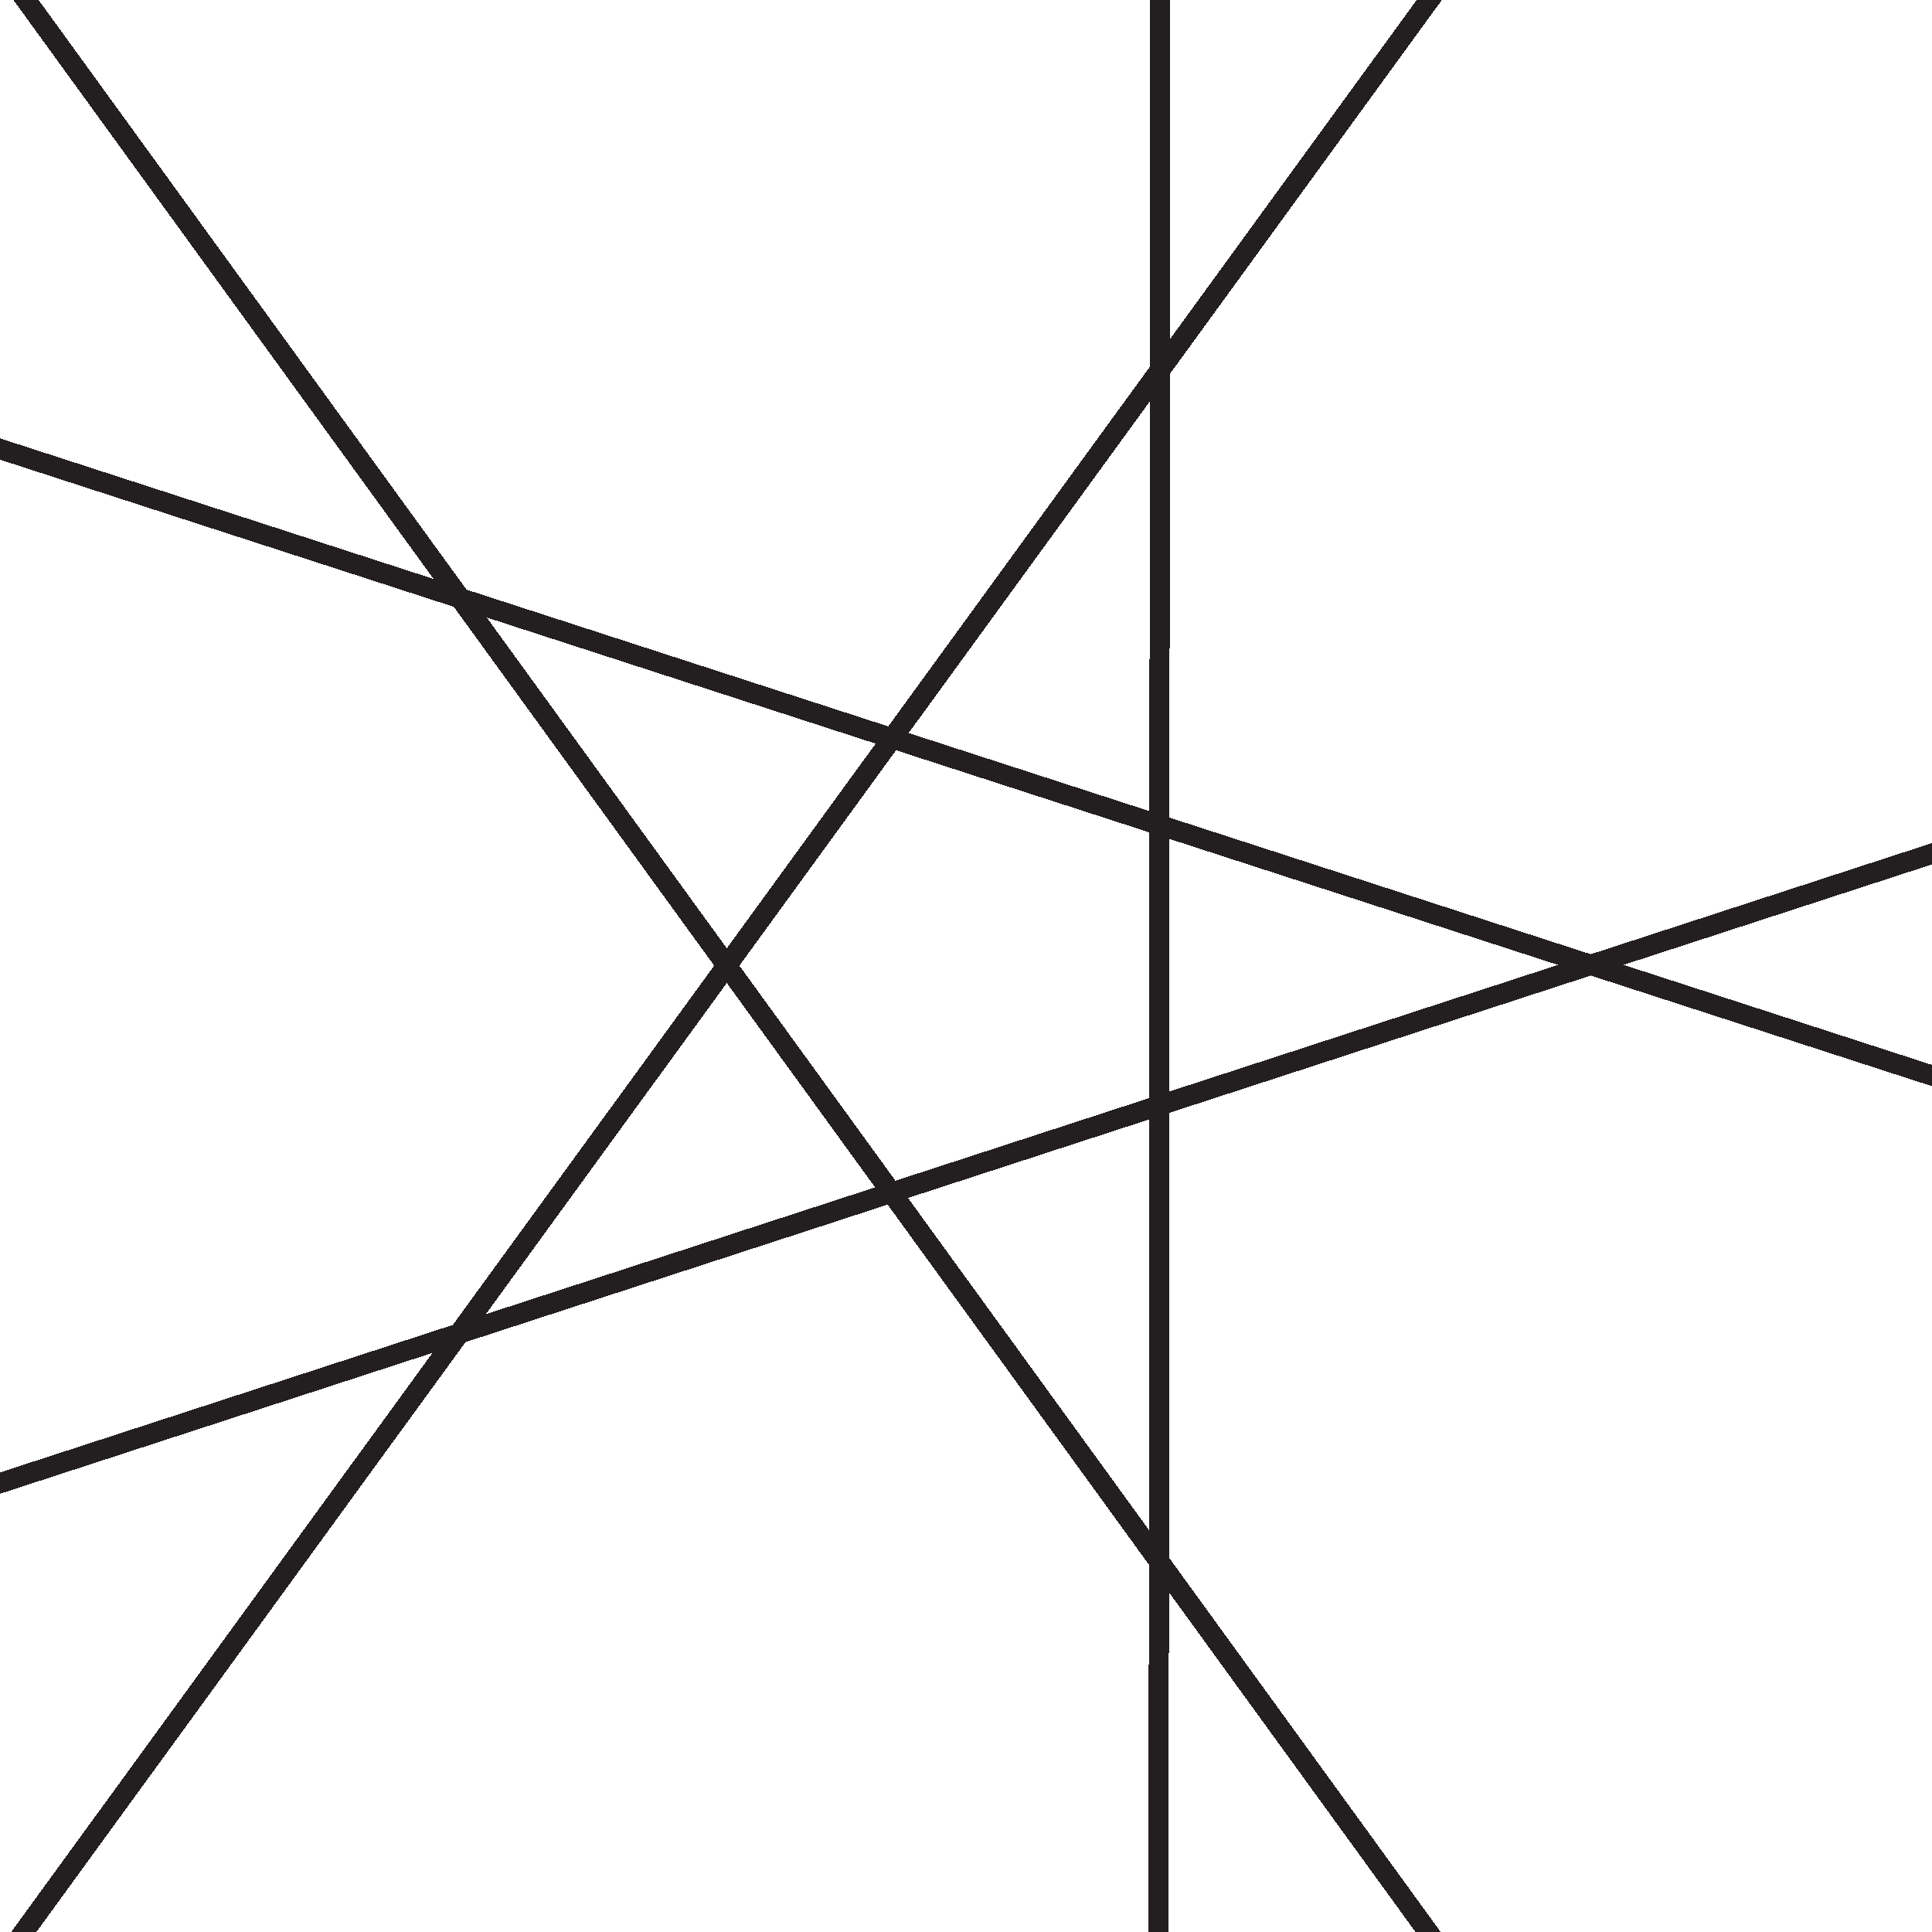
\includegraphics[height=1.2cm]{./../../common/images/rp5.pdf}
      \end{tabular}
    \end{center}
    \vspace*{-0.3em}    
    
    This surface has an equation of the form 
    $S_5(x,y) + t(z)=0,$
    where $S_5(x,y)$ is a regular pentagon (right picture) and $t(z)$ is a
    variant of the Tchebychev polynomials which we already mentioned several
    times.

     Another quintic (left) with $15$ cusps was constructed by
    Wolf Barth; it is related to the Clebsch Cubic (right) as one can see from the
    picture in the middle:

    \vspace*{-0.3em}
    \begin{center}
      \begin{tabular}{c@{\quad}c@{\quad}c}
        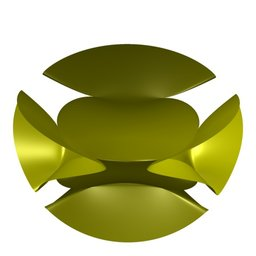
\includegraphics[height=1.2cm]{./../../common/images/barthquintic_green}
        &
        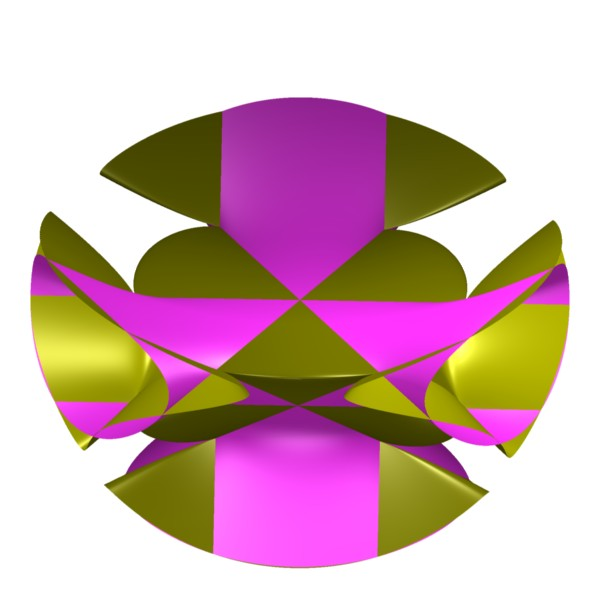
\includegraphics[height=1.2cm]{./../../common/images/barthquintic_clebschcubic}
        &
        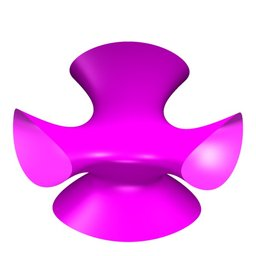
\includegraphics[height=1.2cm]{./../../common/images/clebschcubic_pink}
      \end{tabular}
    \end{center}
    \vspace*{-0.3em}
\end{surferPage}
